\chapter{Efficienza Algoritmica sulle Architetture CPU Moderne}
\label{chap:efficienza-cpu}

\FloatBarrier
\section{Il Ruolo dell'Efficienza nell'Information Retrieval}

Lo sviluppo di sistemi di elaborazione delle informazioni si articola lungo due dimensioni complementari e spesso in tensione tra loro:

\begin{enumerate}
    \item \textbf{Efficacia (\textit{Effectiveness}):} massimizza la soddisfazione dell'utente finale (\textit{user satisfaction}), concentrandosi sulla qualit\`a semantica dei risultati, sul ranking e sull'elaborazione del linguaggio naturale, tipicamente con strumenti ad alto livello di astrazione (Python, framework di Machine Learning).
    \item \textbf{Efficienza (\textit{Efficiency}):} minimizza i costi operativi infrastrutturali, progettando algoritmi ottimizzati fino all'ultimo ciclo di clock della CPU e all'ultimo bit di memoria occupato.
\end{enumerate}

Non \`e richiesto che una singola figura professionale padroneggi entrambi gli estremi; tuttavia chi sviluppa ad alto livello deve comprendere i vincoli fisici dell'hardware sottostante per non progettare soluzioni impraticabili, mentre chi ottimizza a basso livello deve preservare la struttura e la semantica dei dati per non comprometterne l'efficacia.

\subsection{I Tre Pilastri dell'Efficienza nei Sistemi IR}

\paragraph{Esperienza utente.} Nei sistemi web su scala planetaria, la risposta a una query deve essere erogata entro una frazione infinitesima di secondo. L'utente percepisce qualsiasi ritardo superiore a pochi decimi di secondo: se i risultati tardano o risultano irrilevanti, abbandona il servizio a favore della concorrenza. L'efficienza algoritmica non serve solo a rispondere pi\`u rapidamente, ma consente di eseguire algoritmi di ranking e filtraggio pi\`u sofisticati ed efficaci \emph{entro il medesimo budget temporale prestabilito} (tipicamente un tetto massimo di $100$--$200\,\text{ms}$).

\paragraph{Scalabilit\`a operativa.} I sistemi moderni gestiscono miliardi di documenti, elementi multimediali, query e log generati ogni secondo. Il numero di macchine necessarie \`e approssimativamente:
\[
\text{Numero di macchine} = \left\lceil \frac{\text{Volume totale dei dati}}{\text{Capacit\`a operativa del singolo nodo}} \right\rceil.
\]
Se il volume dei dati raddoppia, un sistema ben progettato richiede al pi\`u il doppio delle macchine (scalabilit\`a lineare); un algoritmo inefficiente pu\`o invece richiedere una crescita superlineare dei costi (ad es. quadruplicare i server), insostenibile su larga scala. Per rispettare le latenze richieste, i dati attivi devono risiedere in RAM ed evitare gli accessi a disco: ci\`o richiede algoritmi efficienti non solo in tempo ma anche in spazio, tramite tecniche di compressione. Inoltre, poich\'e i dati vengono replicati su pi\`u macchine per tolleranza ai guasti (\textit{fault tolerance}), ogni inefficienza di memoria viene amplificata dal fattore di replica dell'infrastruttura.

\paragraph{Sostenibilit\`a ambientale ed economica.} La riduzione del numero di macchine fisiche abbatte direttamente il consumo energetico dei data center. I server ad alta densit\`a dissipano ingenti quantit\`a di calore e gran parte dell'energia \`e consumata dagli impianti di raffreddamento; per questo molti data center su larga scala vengono collocati in regioni fredde o vicino a corsi d'acqua (\textit{free cooling}). Un risparmio computazionale marginale, anche solo del $3\%$, genera risparmi economici rilevanti e riduce l'impronta di carbonio.

\FloatBarrier
\section{La Gerarchia di Memoria e i Principi di Localit\`a}

\subsection{Il Divario di Latenza tra CPU e Memoria}

Nel modello teorico computazionale classico (macchina RAM astratta) l'accesso a qualunque locazione di memoria ha costo unitario costante, $\BigO{1}$. Nelle macchine fisiche reali le unit\`a aritmetiche della CPU operano a velocit\`a enormemente superiori rispetto alla memoria principale (DRAM), ed esiste una gerarchia di livelli intermedi (le \textit{cache}) che approssima l'accesso rapido per i dati usati di frequente.

\begin{table}[htbp]
\centering
\small
\begin{tabular}{l r r r}
\toprule
\textbf{Livello hardware} & \textbf{Latenza tipica} & \textbf{Cicli CPU} & \textbf{Capacit\`a tipica} \\
\midrule
Istruzione CPU (ALU) & $0.5$--$5\,\text{ns}$ & $1$--$2$ & registri interni \\
L1I / L1D Cache & $0.5\,\text{ns}$ & $\approx 1$ & $32\,\text{KB}$ per core \\
L2 Cache & $1.5\,\text{ns}$ & $\approx 3$--$4$ & $256\,\text{KB}$ (fino a $2\,\text{MB}$) \\
L3 Cache (LLC) & $5.0\,\text{ns}$ & $\approx 10$--$15$ & $16\,\text{MB}$ (fino a $64\,\text{MB}$+) \\
RAM principale (DRAM) & $80.0\,\text{ns}$ & $\approx 160$--$200$+ & $64\,\text{GB}$+ \\
Disco / Storage & $500\,000\,\text{ns}$ ($0.5\,\text{ms}$) & milioni & $8\,\text{TB}$+ \\
\bottomrule
\end{tabular}
\caption{Confronto quantitativo di latenza e capacit\`a tra i livelli della gerarchia di memoria.}
\label{tab:gerarchia-memoria}
\end{table}

\begin{definition}[Algoritmo \textit{Memory-Bound}]
Un algoritmo che accede alla RAM centrale in modo disordinato paga $\approx 80\,\text{ns}$ per ogni accesso, intervallo in cui la CPU potrebbe eseguire centinaia di istruzioni. L'algoritmo si dice \textbf{memory-bound}: il tempo di esecuzione \`e dominato dall'attesa del trasferimento dati dalla DRAM e la CPU trascorre la maggior parte del tempo in stallo, rendendo irrilevante l'ottimizzazione del numero di operazioni aritmetiche.
\end{definition}

\subsection{Architettura Fisica sul Chip}

La cache L1 \`e integrata a ridosso dell'unit\`a di decodifica e delle unit\`a di esecuzione; per evitare conflitti di bus \`e fisicamente suddivisa in \textbf{L1I} (\textit{Instruction Cache}, contiene il codice macchina prelevato per l'esecuzione) e \textbf{L1D} (\textit{Data Cache}, contiene gli operandi delle istruzioni di \texttt{load}/\texttt{store}). La cache L2 \`e integrata nel singolo core e funge da cuscinetto a bassa latenza; la cache L3 \`e esterna ai singoli core ma interna al package ed \`e condivisa tra tutti i core della macchina.

\begin{noteblock}{La Cache Line come Unit\`a Minima di Trasferimento}
La RAM e la gerarchia di cache non trasferiscono mai singoli byte o singole variabili isolate: l'unit\`a minima di trasferimento hardware \`e la \textbf{cache line}, tipicamente $B = 64$ byte. Se un programma necessita di un intero a 64 bit ($8$ byte) situato all'indirizzo $A$, l'hardware carica forzatamente l'intero blocco allineato
\[
\left[\left\lfloor A / 64 \right\rfloor \times 64,\ \left\lfloor A / 64 \right\rfloor \times 64 + 63\right].
\]
Se il programma legge quell'unico valore e poi salta a un indirizzo casuale, i restanti $56$ byte ($87.5\%$ del traffico di memoria) vengono sprecati.
\end{noteblock}

\subsection{Localit\`a Temporale e Spaziale}

Un programma sfrutta efficacemente la gerarchia di memoria solo se rispetta almeno una delle due forme di localit\`a:

\begin{itemize}
    \item \textbf{Localit\`a temporale:} quando una data locazione di memoria viene acceduta, \`e altamente probabile che la medesima locazione venga acceduta nuovamente nell'immediato futuro. Le politiche di rimpiazzo delle cache (varianti di \textbf{LRU}, \textit{Least Recently Used}) scartano i dati meno recentemente utilizzati per preservare le locazioni accedute di frequente.
    \item \textbf{Localit\`a spaziale:} quando una data locazione di memoria viene acceduta, \`e altamente probabile che locazioni contigue o vicine vengano accedute nell'immediato futuro. Poich\'e l'hardware trasferisce l'intera cache line, l'accesso a elementi contigui ammortizza il costo di caricamento su tutti gli elementi contenuti al suo interno.
\end{itemize}

\subsection{Hardware Prefetcher}

I processori integrano circuiti dedicati, gli \textbf{hardware prefetcher}, il cui compito \`e anticipare le richieste di memoria dell'applicazione:

\begin{itemize}
    \item \textbf{Stream prefetcher:} se un programma scansiona linearmente la memoria da sinistra verso destra ($A, A+64, A+128, \dots$), il circuito rileva il pattern sequenziale e ordina il caricamento preventivo delle cache line successive in L1/L2 prima ancora che il programma emetta l'istruzione di lettura, mascherando cos\`i la latenza.
    \item \textbf{Stride prefetcher:} intercetta accessi a passo costante (\textit{stride}), ad esempio scansioni che campionano la memoria a intervalli fissi; riconosciuto il gradiente costante, carica selettivamente le cache line corrispondenti al passo di salto.
    \item \textbf{Pattern casuali:} di fronte a salti casuali e non deterministici (\textit{pointer chasing}), nessun hardware prefetcher \`e in grado di anticipare gli accessi, causando lo stallo completo della pipeline a ogni lettura.
\end{itemize}

\FloatBarrier
\section{Caso di Studio: Scansione Sequenziale contro \textit{Pointer Chasing}}
\label{sec:pointer-chasing}

Per dimostrare sperimentalmente l'impatto della localit\`a e del prefetching si confrontano due funzioni Rust operanti su un vettore \texttt{v} di dimensione $N$. Il vettore di ingresso rappresenta una \textbf{permutazione casuale con un singolo ciclo} $\pi \in S_N$.

\begin{definition}[Permutazione con un singolo ciclo]
Una permutazione $\pi$ dell'insieme $\{0, 1, \dots, N-1\}$ contiene un singolo ciclo se e solo se, partendo dall'indice $0$, la catena $k_{t+1} = \pi(k_t)$ visita ogni posizione dell'array esattamente una volta prima di tornare a $0$:
\[
0 \to \pi(0) \to \pi(\pi(0)) \to \dots \to \pi^{N-1}(0) \to 0,
\]
senza cicli isolati o sottocicli disgiunti.
\end{definition}

Entrambe le funzioni calcolano la sommatoria di tutti gli elementi del vettore, $\sum_{i=0}^{N-1} v[i] = \frac{(N-1)N}{2}$.

\begin{lstlisting}[style=rustcode,caption={Scansione sequenziale lineare.}]
pub fn sum(v: &[usize]) -> usize {
    let mut sum = 0;
    for &value in v.iter() {
        sum += value;
    }
    sum
}
\end{lstlisting}

\begin{lstlisting}[style=rustcode,caption={Scansione per salti casuali (\textit{pointer chasing}).}]
pub fn sum_by_jumping(v: &[usize]) -> usize {
    let mut sum = 0;
    let mut k = 0;
    for _ in 0..v.len() {
        sum += v[k];
        k = v[k]; // il valore letto diventa l'indice della prossima iterazione
    }
    sum
}
\end{lstlisting}

Nel modello teorico RAM entrambe le funzioni eseguono $N$ iterazioni con un'operazione di somma per passo: hanno cio\`e identica complessit\`a asintotica $\BigO{N}$. Sulla macchina fisica, misurando il tempo medio per singolo elemento al variare della dimensione dell'array, emergono per\`o divergenze marcate.

\begin{table}[htbp]
  \centering
  \small
  \setlength{\tabcolsep}{6pt}
  \begin{tabular}{r r l r r r}
    \toprule
    & & & \multicolumn{2}{c}{\textbf{Tempo per elem.}} & \\
    \cmidrule(lr){4-5}
    \textbf{$N$} & \textbf{Dim.} & \textbf{Livello cache} & \textbf{\texttt{sum()}} & \textbf{\texttt{jumping()}} & \textbf{Rallentamento} \\
    \midrule
    $256$         & $2\,\text{KiB}$   & L1 ($32\,\text{KB}$)  & $0.1\,\text{ns}$ & $1.3\,\text{ns}$  & $13\times$  \\
    $8\,192$      & $64\,\text{KiB}$  & L2 ($256\,\text{KB}$) & $0.1\,\text{ns}$ & $2.5\,\text{ns}$  & $25\times$  \\
    $262\,144$    & $2\,\text{MiB}$   & L3 ($16\,\text{MB}$)  & $0.2\,\text{ns}$ & $13.4\,\text{ns}$ & $67\times$  \\
    $16\,777\,216$& $128\,\text{MiB}$ & RAM (DRAM)            & $0.4\,\text{ns}$ & $84.9\,\text{ns}$ & $212\times$ \\
    \bottomrule
  \end{tabular}
  \caption{Tempo medio per elemento di \texttt{sum()} e \texttt{sum\_by\_jumping()} al variare della dimensione dell'array.}
  \label{tab:pointer-chasing-benchmark}
\end{table}

\subsection{Analisi delle Cause Fisiche}

\paragraph{Perch\'e \texttt{sum()} varia solo da $0.1$ a $0.4\,\text{ns}$?} Con interi \texttt{usize} a 64 bit ($8$ byte), in una cache line da $64$ byte alloggiano $64/8 = 8$ elementi contigui: si ha piena localit\`a spaziale. L'accesso a una nuova linea comporta un miss iniziale, ma i successivi $7$ accessi avvengono a costo pressoch\'e nullo da cache, e lo stream prefetcher carica le linee successive in anticipo rispetto all'esecuzione. Indicando con $T_{\text{comp}}$ il tempo di calcolo e con $T_{\text{load}}$ il tempo di trasferimento ammortizzato, il costo osservato per elemento segue
\[
\text{Latenza osservata} \approx \max\!\left(T_{\text{comp}},\ T_{\text{load\_ammortizzato}}\right),
\]
quasi interamente mascherato dal calcolo; l'aumento da $0.1$ a $0.4\,\text{ns}$ su $128\,\text{MiB}$ \`e dovuto unicamente alla saturazione della banda del bus verso la RAM.

\paragraph{Perch\'e \texttt{sum\_by\_jumping()} arriva a $84.9\,\text{ns}$?} Poich\'e la permutazione \`e casuale, l'indirizzo $k_{t+1} = v[k_t]$ punta a una locazione arbitraria: la probabilit\`a che cada nella stessa cache line \`e trascurabile, quindi per ogni elemento letto da $8$ byte i restanti $56$ byte trasferiti vengono scartati (assenza totale di localit\`a spaziale). Non essendovi passo lineare o costante, il prefetching \`e inibito. Inoltre la CPU deve conoscere l'indice della lettura successiva prima di poterla emettere: si tratta di una \textbf{dipendenza seriale} che impedisce ogni sovrapposizione. Quando la dimensione dell'array supera la capienza della L3 ($128\,\text{MiB} \gg 16\,\text{MB}$), ogni accesso diventa un cache miss globale verso la DRAM:
\[
\text{Tempo per elemento} \approx \text{latenza di accesso fisico alla DRAM} \approx 80\text{--}85\,\text{ns},
\]
valore che coincide esattamente con i $84.9\,\text{ns}$ misurati.

\begin{example}[Ammortizzare il costo del \textit{pointer chasing} sfruttando la cache line]
Se il salto avviene tra blocchi di $64$ byte (8 interi a 64 bit), ma tutti gli elementi del blocco vengono sommati prima del salto successivo, il costo di un cache miss verso la RAM ($\approx 85\,\text{ns}$) viene sostenuto una sola volta ogni $8$ operazioni di somma:
\begin{lstlisting}[style=rustcode]
pub fn sum_by_jumping_cache_lines(v: &[usize]) -> usize {
    let mut sum = 0;
    let mut k = 0;
    let num_blocks = v.len() / 8;
    for _ in 0..num_blocks {
        let base = k * 8;
        // sfrutta appieno la cache line gia' caricata in memoria
        sum += v[base] + v[base + 1] + v[base + 2] + v[base + 3]
             + v[base + 4] + v[base + 5] + v[base + 6];
        k = v[base + 7] % num_blocks; // puntatore al prossimo salto
    }
    sum
}
\end{lstlisting}
La latenza viene ammortizzata su $8$ elementi, portando il tempo medio atteso per valore a
\[
\text{Tempo medio per valore} \approx \frac{85\,\text{ns}}{8} \approx 10.6\,\text{ns},
\]
un risultato intermedio tra la scansione lineare e il salto casuale elemento per elemento.
\end{example}

\begin{remark}[Eliminare il rallentamento residuo di \texttt{sum()}]
Il lieve rallentamento da $0.1$ a $0.4\,\text{ns}$ osservato in \texttt{sum()} si verifica perch\'e $T_{\text{comp}} \approx 0.1\,\text{ns}$ \`e inferiore al tempo necessario ad alimentare il flusso dati dalla RAM su vettori molto grandi (regime memory-bound). Aumentando la complessit\`a computazionale del corpo del ciclo (ad es. moltiplicazioni o funzioni non banali su ciascun elemento) si ottiene $T_{\text{comp}} \gg T_{\text{load\_RAM}}$: la relazione $\max(T_{\text{comp}}, T_{\text{load}})$ diventa costantemente pari a $T_{\text{comp}}$, il regime diventa \textit{CPU-bound} e la curva dei tempi risulta perfettamente piatta al variare di $N$.
\end{remark}

\FloatBarrier
\section{Forme di Parallelismo e Architettura della Pipeline}

Le moderne CPU sfruttano molteplici forme di parallelismo: il \textbf{multi-threading/multi-core} (pi\`u core fisici indipendenti sullo stesso processore), il \textbf{pipelining} (suddivisione dell'esecuzione dell'istruzione in stadi operanti simultaneamente su istruzioni contigue) e l'esecuzione \textbf{superscalare} (unit\`a di calcolo multiple nello stesso core per elaborare pi\`u istruzioni indipendenti per ciclo).

\begin{noteblock}{Parallelismo Triviale nei Motori di Ricerca}
Nei motori di ricerca non \`e necessario sincronizzare pi\`u core per rispondere a una singola query: si adotta il \textbf{parallelismo triviale} (\textit{embarrassingly parallel}), in cui, data la presenza di migliaia di utenti simultanei, ogni thread su un singolo core serve in modo completamente isolato una specifica query. Non essendovi condivisione di stato, si azzerano le contese sui lock e i problemi di coerenza della cache.
\end{noteblock}

\subsection{Anatomia del Pipelining a Cinque Stadi}

Il pipelining scompone l'esecuzione di un'istruzione in stadi sequenziali indipendenti che, in un'architettura standard, sono cinque:

\begin{enumerate}
    \item \textbf{IF} (\textit{Instruction Fetch}): prelievo dell'istruzione in codice macchina dalla memoria (L1I) tramite il \textit{program counter}.
    \item \textbf{ID} (\textit{Instruction Decode}): decodifica dell'istruzione in micro-operazioni ($\mu$-ops) e lettura dei registri sorgente.
    \item \textbf{EX} (\textit{Execute}): esecuzione del calcolo aritmetico-logico nelle ALU o calcolo dell'indirizzo effettivo di memoria.
    \item \textbf{MEM}: accesso al sottosistema di memoria (L1D) per istruzioni di caricamento o scrittura (\texttt{LOAD}/\texttt{STORE}).
    \item \textbf{WB} (\textit{Write-Back}): scrittura del risultato nei registri architetturali e ritiro dell'istruzione.
\end{enumerate}

\begin{figure}[htbp]
\centering
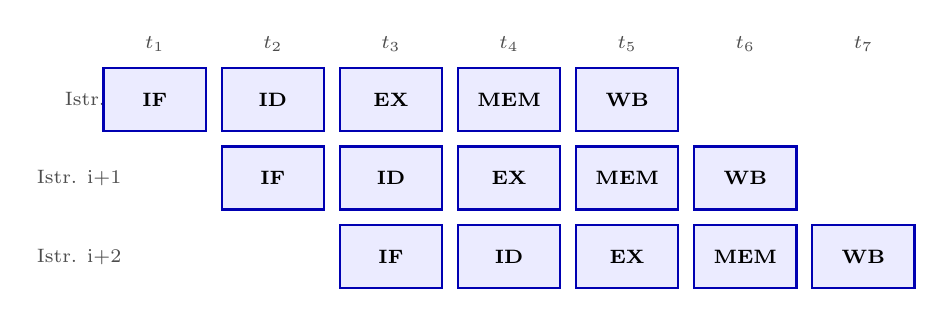
\begin{tikzpicture}[
    stage/.style={rectangle, draw=blue!70!black, fill=blue!8, thick, minimum width=1.3cm, minimum height=0.8cm, align=center, font=\scriptsize\bfseries},
    lbl/.style={font=\scriptsize, text=gray!60!black}
]
    \foreach \i/\name/\y in {0/i/0, 1/i+1/-1, 2/i+2/-2} {
        \node[lbl, anchor=east] at (-0.3, \y) {Istr. \name};
    }
    \foreach \s [count=\c from 0] in {IF,ID,EX,MEM,WB} {
        \node[stage] at (\c*1.5, 0) {\s};
    }
    \foreach \s [count=\c from 1] in {IF,ID,EX,MEM,WB} {
        \node[stage] at (\c*1.5, -1) {\s};
    }
    \foreach \s [count=\c from 2] in {IF,ID,EX,MEM,WB} {
        \node[stage] at (\c*1.5, -2) {\s};
    }
    \node[lbl] at (0, 0.7) {$t_1$};
    \foreach \t [count=\c from 2] in {2,...,7} {
        \node[lbl] at (\c*1.5-1.5, 0.7) {$t_{\c}$};
    }
\end{tikzpicture}
\caption{Sovrapposizione degli stadi della pipeline a 5 stadi su istruzioni consecutive.}
\label{fig:pipeline-5-stadi}
\end{figure}

\subsection{Latenza, Throughput e Profondit\`a della Pipeline}

Sia $k$ il numero di stadi della pipeline e $\tau$ il periodo del ciclo di clock. La \textbf{latenza} $L$ \`e il tempo totale richiesto da una singola istruzione per attraversare l'intera pipeline, $L = k \cdot \tau$: nelle CPU moderne la latenza per un'operazione semplice varia tipicamente tra $10$ e $20$ cicli di clock. Il \textbf{throughput} $W$ \`e il numero di istruzioni completate per unit\`a di tempo e, a regime, $W = 1/\tau$ istruzioni al secondo, poich\'e a ogni ciclo un'istruzione esce dalla pipeline. Il periodo $\tau$ \`e imposto dal ritardo dello stadio pi\`u lento della catena circuitale,
\[
\tau \ge \max_{1 \le i \le k} \left(t_{\text{stadio}_i}\right).
\]
Per innalzare la frequenza di clock (ridurre $\tau$) i progettisti aumentano la profondit\`a $k$ della pipeline (fino a 15--20 o pi\`u stadi nelle CPU moderne), implementando ciascuno stadio con circuiteria pi\`u semplice e veloce; di contro, l'aumento di $k$ dilata la penalit\`a in caso di svuotamento forzato della pipeline.

\FloatBarrier
\section{Esecuzione Superscalare, Interleaving e Conflitti Strutturali}

Un processore si definisce \textbf{superscalare} quando possiede l'abilit\`a architetturale di avviare e completare pi\`u di un'istruzione per ciclo di clock ($IPC > 1$, \textit{Instructions Per Cycle}) all'interno dello stesso core, integrando unit\`a logico-aritmetiche multiple (ALU per interi, moltiplicatori, unit\`a di shift, unit\`a di load/store) servite da porte di emissione parallele (\textit{execution ports}). Architetture reali come Intel Haswell dispongono ad esempio di una coda di decodifica a 56 voci, un \textit{reorder buffer} a 192 voci, una stazione di prenotazione unificata a 60 voci e 8 porte di esecuzione parallele, ciascuna specializzata per classi di operazioni (ALU intere, load/store, unit\`a vettoriali, branch, ecc.).

\subsection{L'Esperimento dell'\textit{Interleaving} Aritmetico}

Si sottopongono a benchmark quattro funzioni Rust che operano su un vettore di interi a 64 bit \texttt{\&[u64]}, accumulando un numero crescente di operazioni indipendenti per iterazione.

\begin{lstlisting}[style=rustcode,caption={Da un'unica riduzione a quattro riduzioni indipendenti per iterazione.}]
pub fn do_stuff(v: &[u64]) -> u64 {
    let mut prod = 1;
    for &value in v.iter() {
        prod *= value;
    }
    prod
}

pub fn do_more_stuff(v: &[u64]) -> (u64, u64) {
    let mut prod = 1;
    let mut sum = 0;
    for &value in v.iter() {
        prod *= value;
        sum += value;
    }
    (prod, sum)
}

pub fn do_more_stuff_2(v: &[u64]) -> (u64, u64, u64) {
    let mut prod = 1;
    let mut sum = 0;
    let mut xor = 0;
    for &value in v.iter() {
        prod *= value;
        sum += value;
        xor ^= value;
    }
    (prod, sum, xor)
}

#[inline]
pub fn do_more_stuff_3(v: &[u64]) -> (u64, u64, u64, u64) {
    let mut prod = 1;
    let mut sum = 0;
    let mut xor = 0;
    let mut or = 0;
    for &value in v.iter() {
        prod *= value;
        sum += value;
        xor ^= value;
        or |= value;
    }
    (prod, sum, xor, or)
}
\end{lstlisting}

\begin{table}[htbp]
\centering
\small
\begin{tabular}{l r}
\toprule
\textbf{Funzione} & \textbf{Tempo per iterazione} \\
\midrule
\texttt{do\_stuff()} (1 operazione) & $0.4\,\text{ns}$ \\
\texttt{do\_more\_stuff()} (2 operazioni) & $0.4\,\text{ns}$ \\
\texttt{do\_more\_stuff\_2()} (3 operazioni) & $0.4\,\text{ns}$ \\
\texttt{do\_more\_stuff\_3()} (4 operazioni) & $0.5\,\text{ns}$ \\
\bottomrule
\end{tabular}
\caption{Tempo per iterazione al crescere del numero di riduzioni indipendenti accumulate.}
\label{tab:interleaving-arithmetic}
\end{table}

\subsection{Sovrapposizione delle Istruzioni e Saturazione delle Porte}

Da una a tre operazioni il tempo resta invariato a $0.4\,\text{ns}$ perch\'e le variabili di accumulo non presentano dipendenze reciproche: $\text{prod}_{t+1} = \text{prod}_t \cdot v[i]$, $\text{sum}_{t+1} = \text{sum}_t + v[i]$, $\text{xor}_{t+1} = \text{xor}_t \oplus v[i]$. Il core superscalare invia contemporaneamente la moltiplicazione, l'addizione e lo XOR a tre porte di esecuzione distinte: le tre operazioni vengono completate nel medesimo ciclo di clock, e il lavoro aggiuntivo \`e svolto a costo nullo.

Con la quarta operazione (\texttt{or}) il tempo sale a $0.5\,\text{ns}$ anzich\'e raddoppiare a $0.8\,\text{ns}$: si tratta di uno \textbf{structural hazard}, poich\'e le unit\`a fisiche disponibili per calcoli logico-aritmetici in parallelo in un singolo ciclo sono sature (solo tre istruzioni di quel tipo possono essere emesse simultaneamente), e una delle quattro operazioni deve attendere. Tuttavia la CPU \textit{out-of-order} non processa le iterazioni come compartimenti stagni: srotola implicitamente la finestra di istruzioni raggruppandole a blocchi di tre, assorbendo l'operazione in eccesso nei cicli successivi e saturando le capacit\`a residue delle porte. L'overhead reale corrisponde quindi a una frazione marginale di ciclo ($\Delta t = +0.1\,\text{ns}$) anzich\'e a un ciclo intero aggiuntivo.

\FloatBarrier
\section{Data Hazard e Dipendenze Seriali}

\begin{definition}[Data Hazard]
Si verifica un \textbf{data hazard} quando un'istruzione necessita di un operando non ancora disponibile poich\'e in fase di calcolo da parte di un'istruzione precedente. Corrisponde a una dipendenza sui dati di tipo \textbf{RAW} (\textit{Read-After-Write}):
\[
\text{Inst}_A:\ R_1 \leftarrow R_2 + R_3 \qquad \Longrightarrow \qquad \text{Inst}_B:\ R_4 \leftarrow R_1 \times R_5,
\]
dove $\text{Inst}_B$ deve rimanere in stallo nella pipeline finch\'e $\text{Inst}_A$ non conclude il calcolo.
\end{definition}

Si consideri un codice che esegue lo stesso numero di operazioni per iterazione della precedente \texttt{do\_more\_stuff\_3}, ma concatenando i dati in una catena stretta:

\begin{lstlisting}[style=rustcode,caption={Catena di dipendenza seriale RAW tra quattro operazioni.}]
pub fn do_more_stuff_4(v: &[u64]) -> (u64, u64, u64) {
    let mut prod = 1;
    let mut sum = 0;
    let mut xor = 0;
    for &value in v.iter() {
        sum += value;  // 1. calcola sum
        prod *= sum;   // 2. dipende strettamente da sum
        xor ^= prod;   // 3. dipende strettamente da prod
        sum += xor;    // 4. dipende da xor e sovrascrive sum per l'iterazione successiva!
    }
    (prod, sum, xor)
}
\end{lstlisting}

A causa della catena RAW, le unit\`a di esecuzione non possono avviare alcun calcolo in parallelo:
\[
\text{Latenza iterazione} = t_{\text{add}} + t_{\text{mul}} + t_{\text{xor}} + t_{\text{add\_feedback}}.
\]
Poich\'e l'ultima operazione aggiorna \texttt{sum} e la prima istruzione dell'iterazione successiva richiede il nuovo valore di \texttt{sum}, la CPU \textit{out-of-order} non pu\`o avviare l'iterazione $t+1$ in anticipo: le unit\`a superscalari restano inutilizzate. Sperimentalmente, contro i $0.5\,\text{ns}$ di \texttt{do\_more\_stuff\_3} (operazioni indipendenti), \texttt{do\_more\_stuff\_4} misura $1.7\,\text{ns}$ per iterazione ($\approx 3.5\times$ pi\`u lento), pur eseguendo lo stesso numero di operazioni aritmetiche.

\subsection{Soluzione Algoritmica: \textit{Interleaving} di Vettori Indipendenti}

Quando occorre eseguire la medesima funzione con dipendenza stretta su due vettori distinti \texttt{V} e \texttt{West}, l'approccio sequenziale tradizionale (\texttt{do\_more\_stuff\_4(V)} seguito da \texttt{do\_more\_stuff\_4(West)}) impiega un tempo complessivo $2T$. Se invece si scrive un'unica funzione che elabora entrambi i vettori all'interno della stessa iterazione, alternando le due catene indipendenti:

\begin{lstlisting}[style=rustcode,caption={Fusione (interleaving) di due catene RAW indipendenti tra loro.}]
for i in 0..n {
    // catena per V (occupa le porte al ciclo k)
    sum_v += v[i];
    prod_v *= sum_v;
    xor_v ^= prod_v;
    sum_v += xor_v;
    // catena per West, completamente indipendente da V!
    sum_w += west[i];
    prod_w *= sum_w;
    xor_w ^= prod_w;
    sum_w += xor_w;
}
\end{lstlisting}

il tempo di esecuzione misurato \`e identico a quello del solo vettore \texttt{V} ($\approx T$, anzich\'e $2T$). Le operazioni su \texttt{West} non dipendono da quelle su \texttt{V}: mentre la catena di \texttt{V} \`e in attesa dei risultati delle ALU, le unit\`a di calcolo libere processano la catena di \texttt{West}, saturando a costo nullo i tempi morti imposti dalle dipendenze sui dati.

\FloatBarrier
\section{Control Hazard, Esecuzione Speculativa e Branch Prediction}

\begin{definition}[Control Hazard]
Si verifica un \textbf{control hazard} quando la CPU non pu\`o determinare quale sia la successiva istruzione da prelevare dalla memoria (\textit{instruction fetch}) a causa della presenza di un salto condizionato (\texttt{if}, \texttt{branch}).
\end{definition}

La CPU non pu\`o fermarsi a ogni condizione: adotta pertanto l'\textbf{esecuzione speculativa}, ipotizzando tramite un \textit{branch predictor} quale ramo verr\`a imboccato e prelevando speculativamente le istruzioni successive per alimentare la pipeline. Se l'esito della condizione si rivela discorde rispetto alla predizione, tutto il lavoro speculativo completato negli stadi intermedi deve essere annullato, con uno svuotamento completo della pipeline (\textit{pipeline flush}) e il ricaricamento dal ramo corretto:
\[
\text{Penalit\`a per mispredizione} = 15\text{--}20 \text{ cicli di clock}.
\]

\subsection{Il Paradosso della Condizione Casuale}

Si introduce un filtro condizionale in un codice con catena di dipendenza, operando su un array di interi casuali uniformemente distribuiti in $[0, 99]$:

\begin{lstlisting}[style=rustcode,caption={Ramo condizionale su valori casuali: la CPU non pu\`o predire l'esito.}]
pub fn do_more_stuff_5(v: &[u64]) -> (u64, u64, u64) {
    let mut prod = 1;
    let mut sum = 0;
    let mut xor = 0;
    for &value in v.iter() {
        if value > 50 { // vera con p = 0.5 su valori casuali in [0, 99]
            sum += value;
            prod *= sum;
            xor ^= prod;
            sum += xor;
        }
    }
    (prod, sum, xor)
}
\end{lstlisting}

Poich\'e la condizione \`e vera in media il $50\%$ delle volte, ci si aspetterebbe intuitivamente un tempo pressoch\'e dimezzato rispetto a \texttt{do\_more\_stuff\_4} ($1.7 / 2 \approx 0.85\,\text{ns}$). Il tempo misurato sale invece a $3.5\,\text{ns}$, pi\`u del doppio pi\`u lento della versione priva di condizione.

\begin{alertblock}{Il Costo Reale non \`e il Calcolo ma la Mispredizione}
Con valori casuali il branch predictor ha accuratezza pari al lancio di una moneta, $P(\text{hit}) = P(\text{miss}) = 0.50$. Il costo medio per iterazione \`e allora
\[
\begin{aligned}
  \text{Costo medio} &\approx 0.5 \times T_{\text{corpo}} + P(\text{miss}) \times \text{Penalit\`a flush} \\
                     &\approx 0.5 \times 0.85\,\text{ns} + 0.5 \times 5.0\,\text{ns} \approx 2.9\text{--}3.5\,\text{ns},
\end{aligned}
\]
avendo assunto una penalit\`a di $15$--$20$ cicli ($\approx 4$--$5\,\text{ns}$ su una CPU a $4\,\text{GHz}$). Il costo dell'algoritmo non \`e pi\`u dettato dalle operazioni aritmetiche, ma \`e dominato dal tempo perso a svuotare e ricaricare la pipeline.
\end{alertblock}

\subsection{Verifica Sperimentale: Ordinamento dei Dati e Pattern Periodici}

Per dimostrare che il rallentamento deriva esclusivamente dal comportamento del branch predictor, si esegue lo stesso identico codice modificando solo la disposizione dei dati nell'array.

\begin{table}[htbp]
  \centering
  \small
  \setlength{\tabcolsep}{5pt}
  \begin{tabularx}{\textwidth}{l r Y}
    \toprule
    \textbf{Configurazione} & \textbf{Tempo / iter.} & \textbf{Comportamento del predittore} \\
    \midrule
    \texttt{do\_more\_stuff\_4()} (nessun \texttt{if}) & $1.7\,\text{ns}$ & --- \\
    \texttt{do\_more\_stuff\_5()} (dati casuali)       & $3.5\,\text{ns}$ & Ramo impredicibile, miss rate $\approx 50\%$ \\
    \texttt{do\_more\_stuff\_5()} (dati ordinati)      & $1.2\,\text{ns}$ & Predizione quasi perfetta, un solo miss \\
    \texttt{do\_more\_stuff\_5()} (dati alternati)     & $1.1\,\text{ns}$ & Sequenza periodica, miss rate $\approx 0\%$ \\
    \bottomrule
  \end{tabularx}
  \caption{Tempo per iterazione di \texttt{do\_more\_stuff\_5()} al variare della disposizione dei dati.}
  \label{tab:branch-prediction-benchmark}
\end{table}

Con \textbf{dati ordinati} (tutti gli elementi $\le 50$ all'inizio dell'array e tutti quelli $> 50$ alla fine) il predittore assume che il salto non sia preso per l'intera prima met\`a e che sia preso per la seconda: si verifica un unico misprediction al punto di transizione, e rimosso il costo dei flush il tempo scende a $1.2\,\text{ns}$, inferiore ai $1.7\,\text{ns}$ della versione senza condizione poich\'e met\`a delle iterazioni non esegue il corpo dell'\texttt{if}. Con \textbf{dati alternati} secondo un pattern periodico (\textit{falso, vero, falso, vero, \ldots}), i predittori integrano tabelle storiche dei pattern (\textit{branch history shift register}): identificata la periodicit\`a, il predittore anticipa l'esito a ogni passo senza errori, annullando gli stalli.

\subsection{Tecniche \textit{Branchless} e il Salto Implicito dei Cicli \texttt{for}}

Se i dati non sono ordinabili n\'e predicibili, l'unica soluzione consiste nel rimuovere fisicamente il salto condizionale (\textit{branchless code}), sostituendolo con espressioni algebriche o istruzioni condizionali assembly (\texttt{CMOV}). Ad esempio, invece di
\begin{lstlisting}[style=rustcode]
if value > 50 {
    sum += value;
}
\end{lstlisting}
si mappa la guardia logica su un valore binario scalare ($0$ o $1$), eseguendo sempre l'operazione aritmetica:
\begin{lstlisting}[style=rustcode]
let condition = (value > 50) as u64; // vale 1 se vero, 0 se falso
sum += value * condition;            // somma 'value' se vero, somma '0' se falso
\end{lstlisting}
Il programma compie sempre il calcolo matematico, ma il flusso di istruzioni \`e lineare: non vi sono salti, e le mispredizioni sono azzerate.

\begin{remark}[Perch\'e il salto del ciclo \texttt{for} non costituisce un problema]
Ogni ciclo \texttt{for} si conclude a livello macchina con un salto condizionato all'inizio del blocco. Questo branch non degrada le prestazioni perch\'e \`e altamente asimmetrico: per $N$ iterazioni la condizione di permanenza nel ciclo risulta vera per $N-1$ volte consecutive ed \`e falsa solo all'uscita. Il branch predictor impara immediatamente il pattern (``salto preso'') e commette un unico errore di predizione al termine del ciclo, con un impatto del tutto trascurabile sul tempo complessivo.
\end{remark}

\FloatBarrier
\section{Sintesi: dai Vincoli Hardware alle Scelte Algoritmiche}

I fenomeni analizzati in questo capitolo -- gerarchia di memoria e localit\`a, pipelining, esecuzione superscalare, \textit{data hazard} e \textit{control hazard} -- non sono dettagli implementativi trascurabili, ma vincoli fisici che determinano il reale comportamento prestazionale degli algoritmi di Information Retrieval su larga scala. In particolare:

\begin{itemize}
    \item le strutture dati (posting list, indici invertiti) vanno progettate privilegiando l'accesso sequenziale e contiguo, per sfruttare la localit\`a spaziale e l'hardware prefetching;
    \item quando possibile, conviene esprimere pi\`u riduzioni indipendenti all'interno dello stesso ciclo per saturare le porte di esecuzione superscalari a costo marginale;
    \item le catene di dipendenza strette (RAW) tra variabili di accumulo vanno identificate e, se possibile, disaccoppiate o intrecciate (\textit{interleaving}) con calcoli indipendenti;
    \item i rami condizionali imprevedibili sui dati vanno eliminati con tecniche \textit{branchless} o mitigati riordinando i dati per favorire la predizione.
\end{itemize}

La trattazione della vettorizzazione SIMD e degli strumenti di analisi del codice compilato (\textit{Compiler Explorer}) \`e rimandata a un capitolo successivo.
